\section{Evaluation}
This section will focus on critically evaluating the overall project and the performance of the team, outlining strengths and weaknesses of the group work, discussion of whether all the requirements met and as well as learning outcomes and future work. 

\subsection{Teamwork Evaluation}

Achieving a good and productive teamwork is the goal of many organizations nowadays. When looking at the successful projects, it is evident that there is a strong teamwork behind it. However, achieving such a teamwork is not always straightforward. In order to be able to evaluate our work critically, it is crucial to understand characteristics of an effective teamwork in the first place. "The most effective teamwork happens when individual contributors harmonize their efforts and work toward a common goal"\cite{wmtwe}. According to Demand Media, the main characteristics of an effective team work are as following:

\begin{itemize}
\item Good leadership
\item Adaptability
\item Diversity
\item Effective Communication
\item Skilled Conflict Management ( Demand Media, 2015)
\end{itemize} 

Although the overall performance of our group was satisfying, the team lacked some of the qualities of a good teamwork. When evaluating the qualities of our team, we noticed that we had all the 5 characteristics with some minor issues. Lacking a good time management and control system originated several problems such as delays in producing tasks on time. However, having a good communication and conflict solving mechanism helped to overcome those obstacles. One of the vital aspects to be successful is to fully understand strengths and weaknesses of the team.  To have a better view on evaluation of the work throughout the project, we produced full list of our strengths and weaknesses:\newline

\textbf{Strengths}
\begin{itemize}
\item Effective communication - Having a good communication amongst team members was one of the aspects that helped to boost our performance. Every team member was easily reachable through variety of channels including Whatsapp, Skype and Facebook. 
\item Enthusiasm -  Every team member had been very enthusiastic about the project, which in its turn helped everyone to work towards the common goal.
\item Adaptability - This helped the team to overcome obstacles that were caused by choosing inappropriate development model in the beginning of the project and enabled us to quickly adapt more appropriate model.
\item Effective Conflict Solving mechanism - Conflicts in a team work are inevitable and our project wasn't and exception. One of the main conflicts arose between 2 programmers when they had different approach and view on implementation. However a good communication and conflict solving skills help to resolve it swiftly.
\item Diversity - Having team members skilled and experienced in different areas has played a key role to develop each field of the project in parallel.
\end{itemize}  


\textbf{Weaknesses:}
\begin{itemize}
\item Time management -  Having a poor time management have caused delays in producing tasks on time and falling behind the work plan towards the end of project. Although team managed to meet the requirements by working harder towards the end of the project, time management is one area that needs improvement.
\item Role allocation fault - Designating testing role to non-programmers was a naive mistake that was made during the initial stages. This put members with less programming experience in a desperate situation and caused delays in progression of the implementation. Involvement of programmers in this task resolved the problem.
\item Poor meeting management -  One of the weak sides of the team was long and less productive meetings. Having a proper and precise agendas for each meeting could have achieved shorter and better meetings.
\item Stubbornness - Stubbornness is an issue that many team project's suffer, causing diversion from working towards the common goal. This issue, however, had been ruled out half way through the project which boosted the performance in the later stages of the development.
\end{itemize}  

\subsection{Requirements evaluation}
  The purpose of the requirements evaluation is to check whether the team has achieved its goals set in the initial stage. Evaluation proved that project have successfully managed to meet the high priority requirements. Implementation of the lower priority requirements were subject to available time. Hence, they remain unachieved due to strict time constraint. Nevertheless, those requirements will be implemented in the future and are part of the future work plan. Scalable design of the software will allow developers to add even more advanced features to the simulation. Tables below highlight all the functional and non-functional requirements that have been implemented.

\begin{figure}[H]
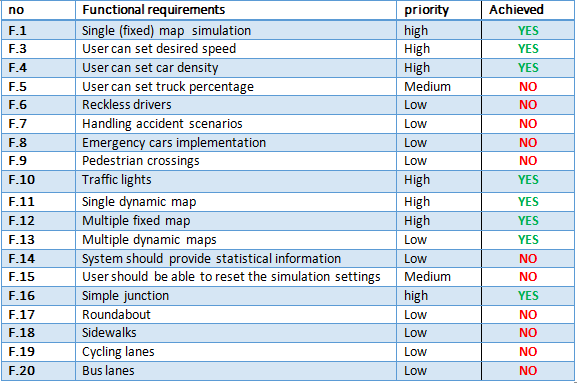
\includegraphics[width=14cm, height=10cm]{pics/FR_EVAL}
\centering
\caption{Functional Requirements evaluation}
\end{figure}


\begin{figure}[H]
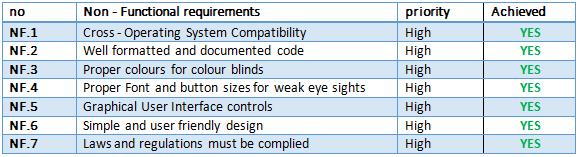
\includegraphics[width=14cm, height=4cm]{pics/NFR_EVAL}
\centering
\caption{Non-Functional Requirements evaluation}
\end{figure}

\subsection{Learning Outcomes}
Getting involved in this project has been very beneficial to every team member in different ways. First of all, the project resembled the real life workplace environment, thus it was very valuable experience and preparation for the future life. Besides that, team members also improved their technical and non-technical skills. One of the most important learning outcomes of the project was understanding the importance of the team work. It gave us the idea of an effective team and how it can be achieved.


